\chapter{Системийн зохиомж}

\begin{figure}[h]
  \centering
  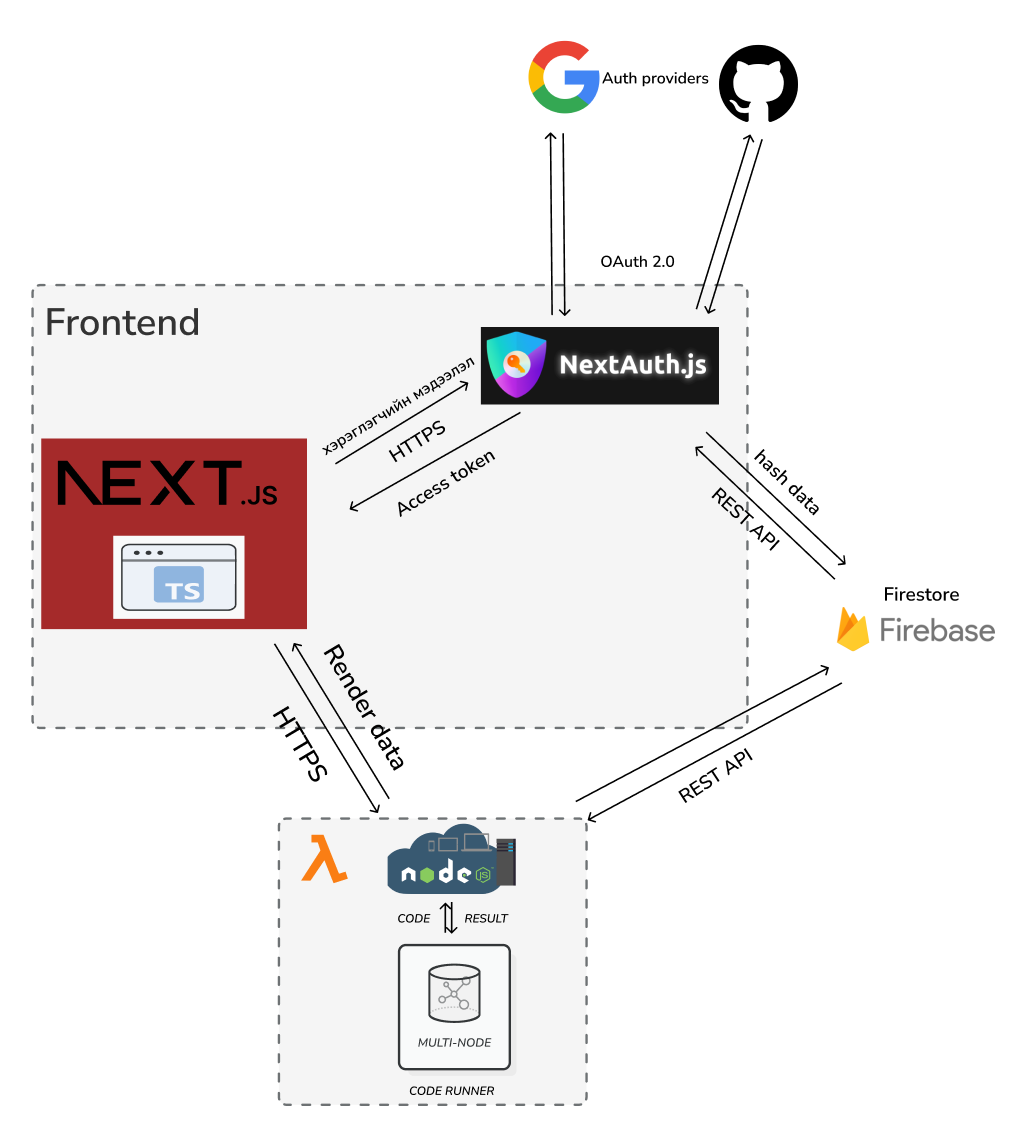
\includegraphics{img/diagrams/architecture.PNG}
  \caption{Системийн ерөнхий зураглал}
\end{figure}

"Coldbrains" системийн ашиглаж буй технологиуд болон тэдгээрийн холбоог харуулж байгаа бөгөөд аль болох ерөнхий байдлаар дүрслэхийг оролдов.

\clearpage

\section{Ажлын явцын диаграм}

\begin{figure}[h]
  \centering
  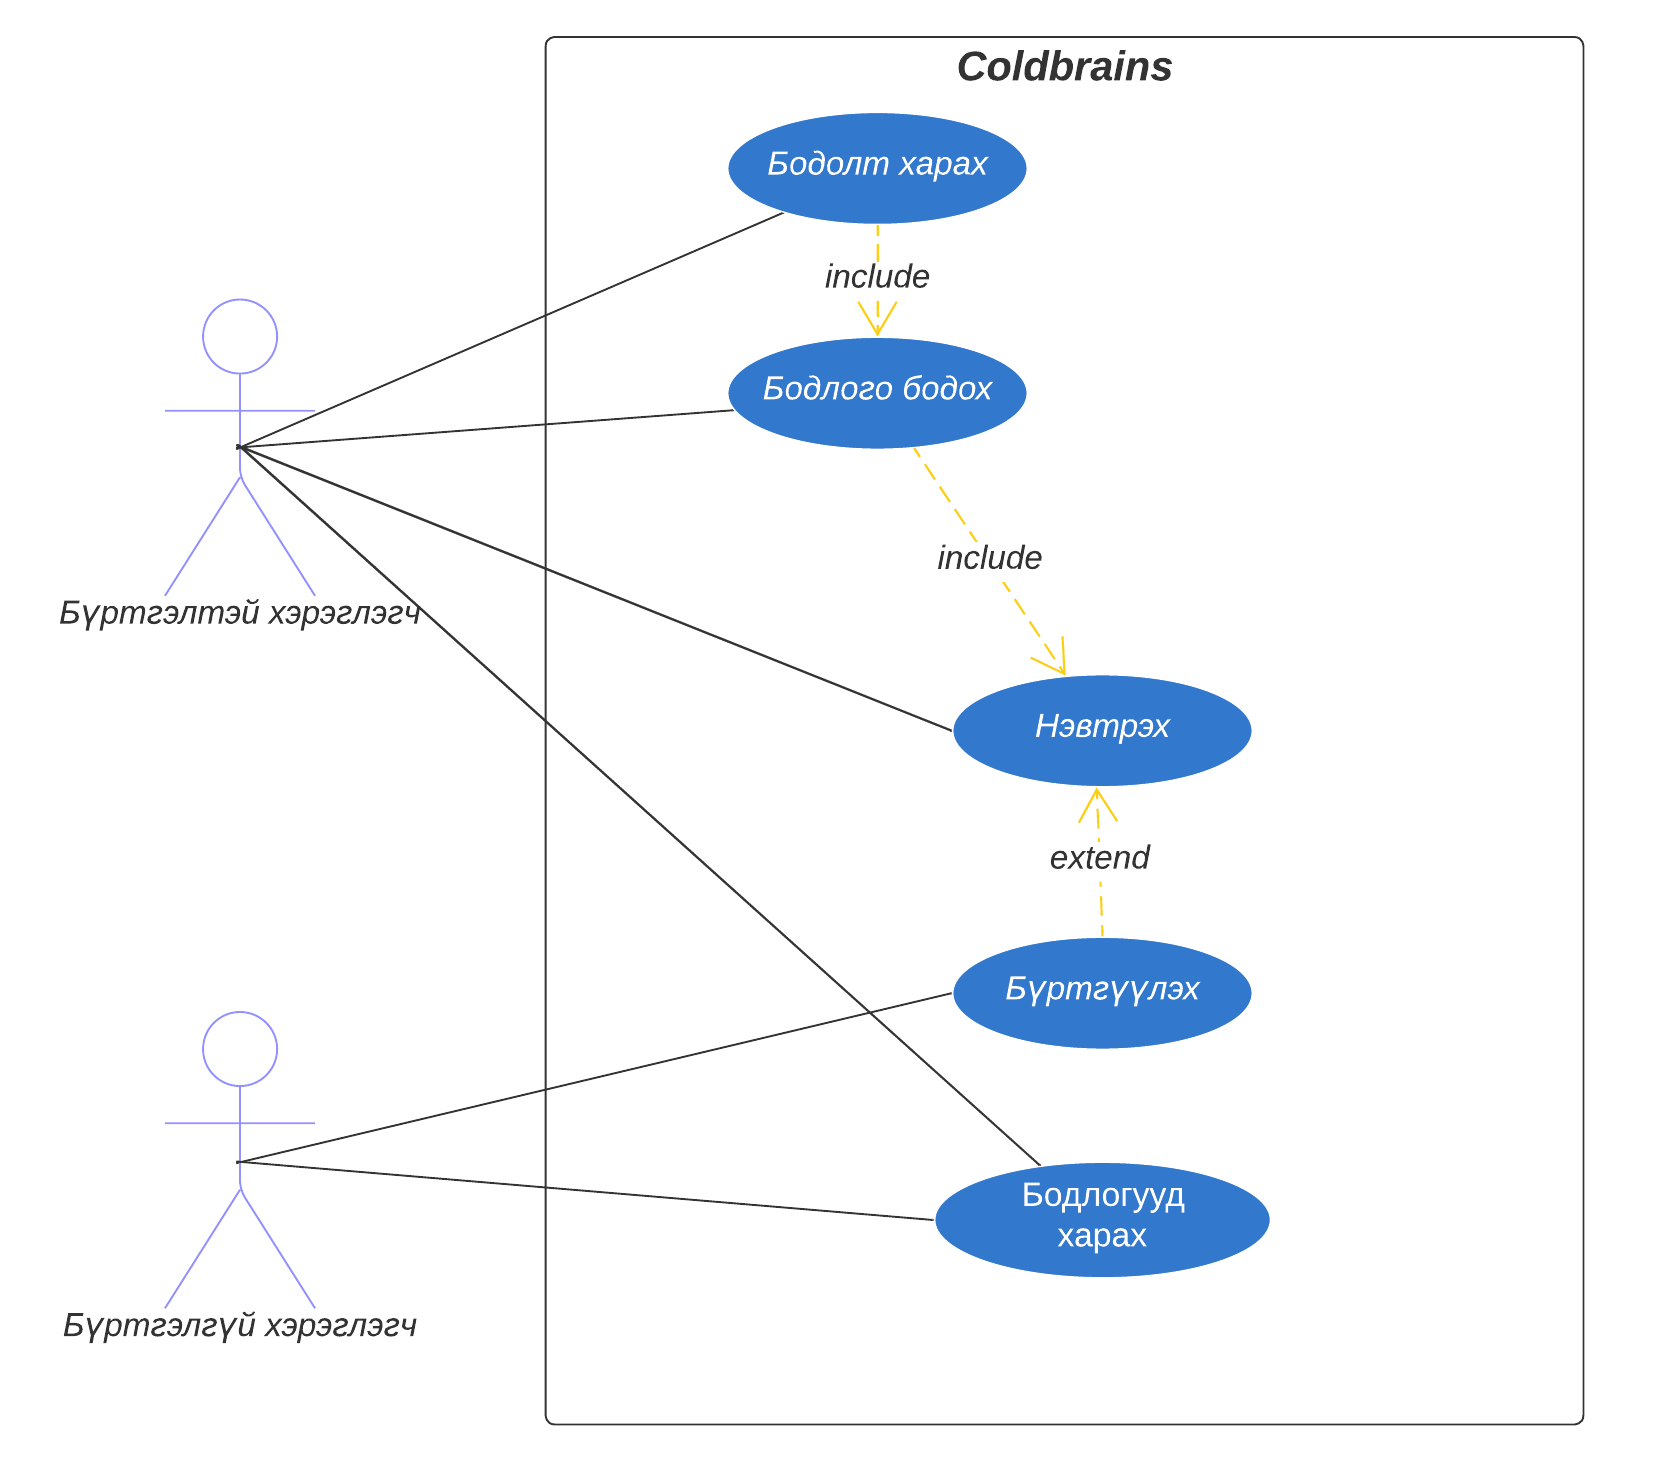
\includegraphics{img/diagrams/coldbrains-use-case.png}
  \caption{Ажлын явцын диаграм}
\end{figure}

Хэрэглэгчийг бүртгэлтэй болон бүртгэлгүй гэж ангилвал бүртгэлгүй хэрэглэгч нь системтэй танилцах зорилгоор бодлогуудын жагсаалтыг харах боломжтой бол бүртгэлтэй хэрэглэгч нь тухайн бодлогуудыг бодох, амжилттай бодсон бол бодолтуудыг харах, мөн өөрийн профайл хэсгийг харах боломжтой болно.

\clearpage

\textbf{Ажлын явц:} 1. Бүртгүүлэх
\begin{table}[H]
  \begin{tabular}{|p{3cm}|p{13.5cm}|}
  \hline
  \multicolumn{1}{|c|}{Ажлын явц}                                       & \multicolumn{1}{c|}{Бүртгүүлэх}                                                                                                                                    \\ \hline
  Зорилго                                                                                       & Тоглогч системд бүртгэл үүсгэж нэвтрэхэд ашиглах                                                                                                                                           \\ \hline
  Угтвар нөхцөл                                                         & Тоглогч систем рүү хандсан байх                                                                                                                                                            \\ \hline
  Тоглогч                                                                                       & Coldbrains системд бүртгэлгүй хэрэглэгч   \\ \hline
  Тайлбарлалт                                                                                   & \begin{tabular}[c]{@{}l@{}}1. Систем нэр, нууц үг, и-мейл хаягийг шаардана.\\ 2. Шаардлагатай мэдээллийг оруулна.\\ 3. Систем амжилттай бүртгэн нэвтрэх хуудас луу шилжүүлнэ.\end{tabular} \\ \hline
  Өргөтгөл                                                                                      & Тоглогч буцах товч даран ажлын явцыг дуусгавар болгоно.                                                                                                                                    \\ \hline
  Хувилбар                                                                                      & 2a. Бүртгэлтэй хэрэглэгч байвал мэдэгдэж, мэдээллийг нь арилгана. Ажлын явцыг эхнээс нь эхлүүлнэ.                                                                                          \\ \hline
  \end{tabular}
\end{table}

\textbf{Ажлын явц:} 2. Бодлогууд харах
\begin{table}[H]
  \begin{tabular}{|p{3cm}|p{13.5cm}|}
  \hline
  \multicolumn{1}{|c|}{Ажлын явц}                                       & \multicolumn{1}{c|}{Бодлогууд харах}                                                                                                                                    \\ \hline
  Зорилго                                                                                       & Тоглогч системд буй бодлогын санг харах                                                                                                   \\ \hline
  Угтвар нөхцөл                                                         & Тоглогч систем рүү хандсан байх                                                                                                                                                   \\ \hline
  Тоглогч                                                                                       & Coldbrains систем рүү хандсан хэрэглэгч                                                                                                                                              \\ \hline
  Тайлбарлалт                                                                                   & \begin{tabular}[c]{@{}l@{}}1. Систем бодлогын санг хэрэглэгчид харуулна.\end{tabular} \\ \hline
  \end{tabular}
\end{table}

\clearpage

\textbf{Ажлын явц:} 3. Нэвтрэх
\begin{table}[H]
  \begin{tabular}{|p{3cm}|p{13.5cm}|}
  \hline
  \multicolumn{1}{|c|}{Ажлын явц}                                       & \multicolumn{1}{c|}{Нэвтрэх}                                                                                                                                    \\ \hline
  Зорилго                                                                                       & Тоглогч системийг ашиглахын тулд нэвтрэх                                                                                                            \\ \hline
  Угтвар нөхцөл                                                         & Тоглогч бодлогын тодорхойлолтыг харах, бодлого бодохыг оролдох,                                                                                                                                                   \\ \hline
  Тоглогч                                                                                       & Coldbrains системд бүртгэлтэй аль эсвэл шууд нэвтрэх сонирхолтой гадны платформд бүртгэлтэй хэрэглэгч                                                                                                                                                                                   \\ \hline
  Тайлбарлалт                                                                                   & \begin{tabular}[c]{@{}l@{}}1. Систем бүртгэлтэй нэр, нууц үг шаардана.\\ 2. Шаардлагатай мэдээллийг оруулна.\\ 3. Систем тоглогчид session үүсгэн бодлогууд хуудас руу шилжүүлнэ.\end{tabular} \\ \hline
  Өргөтгөл                                                                                      & Тоглогч буцах товч даран ажлын явцыг дуусгавар болгоно.                                                                                                                                    \\ \hline
  Хувилбар                                                                                      & 
  1a. Хэрэглэгч бусад платформуудын эрхийг оруулан session үүсгэж ажлын явцыг дуусгана.\newline 2a. Бүртгэлтэй хэрэглэгч олдоогүй бол мэдэгдэж, мэдээллийг нь арилгана. Ажлын явцыг эхнээс нь эхлүүлнэ.                                                                                          \\ \hline
  \end{tabular}
\end{table}

\textbf{Ажлын явц:} 5. Бодолт харах
\begin{table}[H]
  \begin{tabular}{|p{3cm}|p{13.5cm}|}
  \hline
  \multicolumn{1}{|c|}{Ажлын явц}                                       & \multicolumn{1}{c|}{Бодолт харах}                                                                                                                                    \\ \hline
  Зорилго                                                                                       & Тоглогч бодсон бодолгынхоо аргуудаас суралцах зорилгоор бусдын бодолтуудыг харах                                                                                                       \\ \hline
  Угтвар нөхцөл                                                         & Тоглогч тухайн бодлогыг бодсон байх                                                                                                                                                   \\ \hline
  Тоглогч                                                                                       & Системд нэвтэрч орон session үүсгэсэн хэрэглэгч      \\ \hline
  Тайлбарлалт                                                                                   & \begin{tabular}[c]{@{}l@{}}1. Систем тухайн бодлогын бодолтуудыг өөрийн бодолтын хамт харуулна.\\ 2. Тухайн бодолтуудын ямар хэл болон ажилласан хугацааг харуулна.\end{tabular} \\ \hline
  \end{tabular}
\end{table}

\clearpage

\textbf{Ажлын явц:} 4. Бодлого бодох
\begin{table}[H]
  \begin{tabular}{|p{3cm}|p{13.5cm}|}
  \hline
  \multicolumn{1}{|c|}{Ажлын явц}                                       & \multicolumn{1}{c|}{Бодлого бодох}                                                                                                                                    \\ \hline
  Зорилго                                                                                       & Тоглогч системийн бодлогын сангаас бодлого сонгож бодон тухайн бодлогын талаар суралцах, бусдаас шийдлүүдийг сурч авах                                                              \\ \hline
  Угтвар нөхцөл                                                         & Системд нэвтэрч орон бодлогоо сонгосон байх.  \\ \hline
  Тоглогч                                                                                       & Системд нэвтэрч орон session үүсгэсэн хэрэглэгч                            \\ \hline
  Тайлбарлалт                                                                                   & \begin{tabular}[c]{@{}l@{}}1. Систем хэрэглэгчид бодлогын тодорхой тайлбар болон жишээ оролт\\ болон гаралтыг харуулна.\\ 2. Систем оролтод ашиглах boilerplate\footnotemark{} код бүхий код засварлагчийг\\ үүсгэж өгнө.\\ 3. Тоглогч тухайн бодлогын бодолт бүхий кодыг бичнэ.\\ 4. Тоглогч тухайн кодыг ажиллуулах товчийг дарна.\\ 5. Тоглогч тухайн бодлогын бодолтууд хуудас руу шилжинэ.\end{tabular} \\ \hline
  Өргөтгөл & 4b. Тоглогч кодоо дахин засварлаж дараагийн алхмаа хийнэ.\newline 2a. Тоглогч өөрийн дуртай код засварлагчийн загваруудаас сонгоно. \newline 1b. Тоглогч өөрийн мэддэг програмчлалын хэлээ сонгоно.   \\ \hline
  Хувилбар                                                                                      & 
  4a. Тоглогчийн кодын алдааны мэдээлэл болон харгалзах тест кейсийг систем харуулан ажлын явц үргэлжлэнэ.                                                                    \\ \hline
  \end{tabular}
\end{table}
\footnotetext{Ерөнхий хүрээнд ашиглах боломжтой, өөрчлөлт оруулж болох бүхий код}

\clearpage

\textbf{Хэрэглэгчийн кодыг тест кейс дээр ажиллуулан дүгнэх}
\begin{figure}[h]
  \centering
  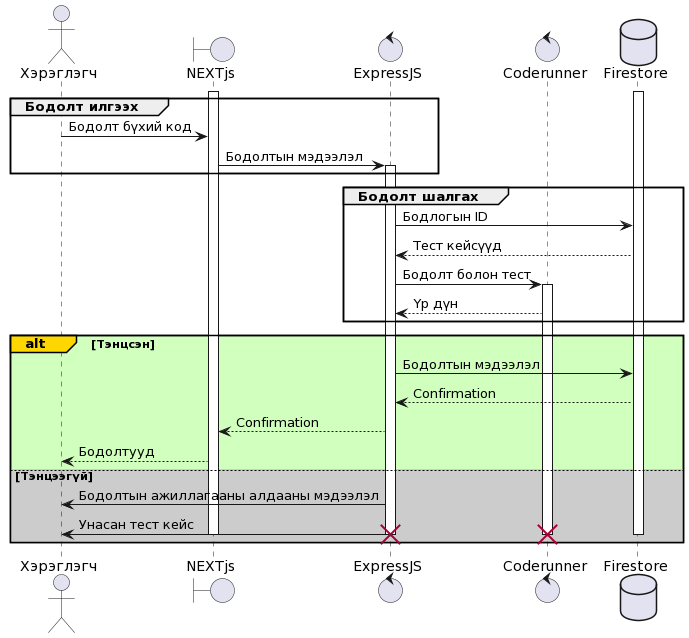
\includegraphics[width=15cm]{img/diagrams/sequence.png}
  \caption{Хэрэглэгчийн кодыг дүгнэж буй сценарийн дарааллын диаграм}
\end{figure}

\clearpage

\section{Хэрэглэгчийн интерфейс}
\subsection{Wireframe}
\begin{figure}[h]
  \centering
  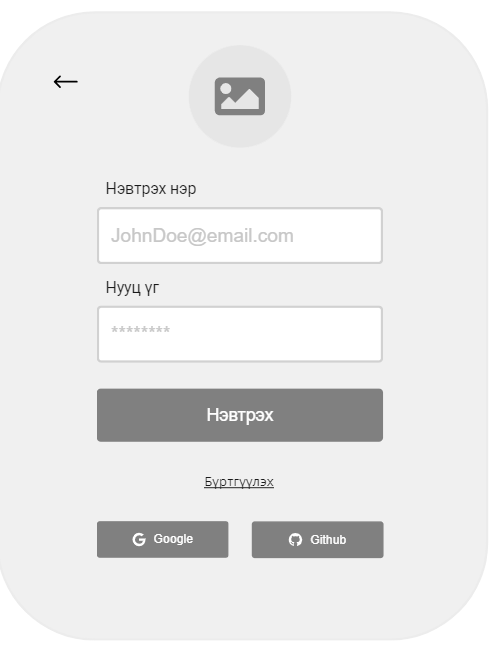
\includegraphics[width=5cm]{img/wireframe/login.PNG}
  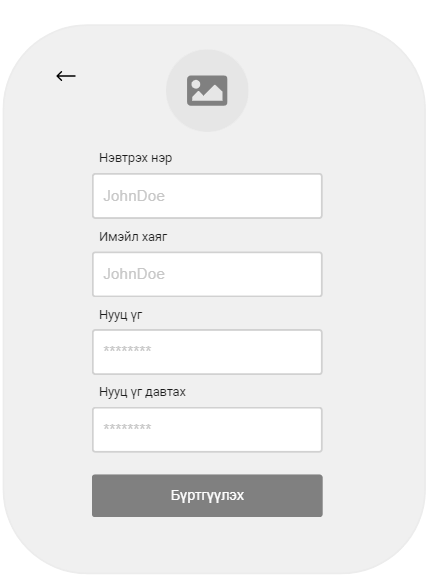
\includegraphics[width=5cm]{img/wireframe/register.PNG}
  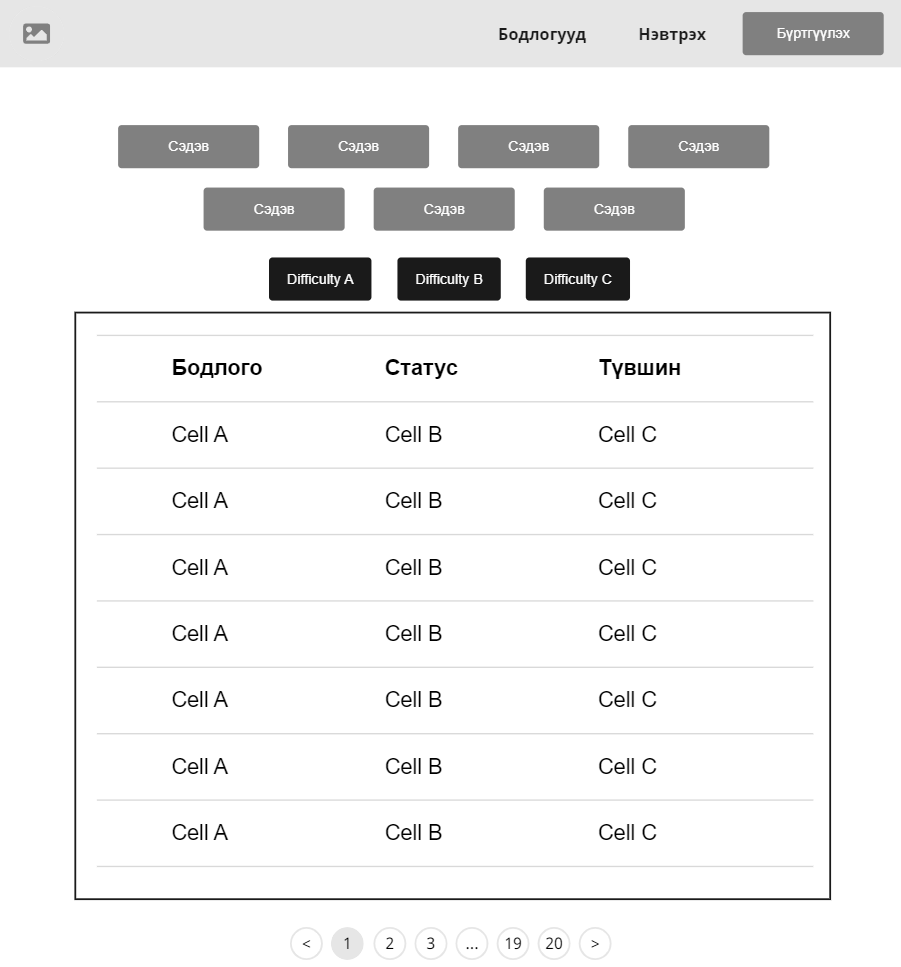
\includegraphics[width=5cm]{img/wireframe/problems.PNG}
  \caption{Wireframe}
\end{figure}

\subsection{Mockup дизайн}
\begin{figure}[h]
  \centering
  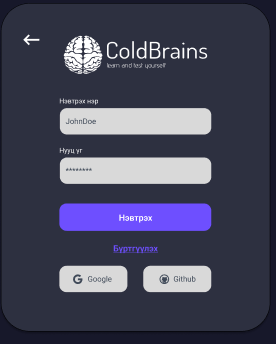
\includegraphics[width=5cm]{img/mockup/login.PNG}
  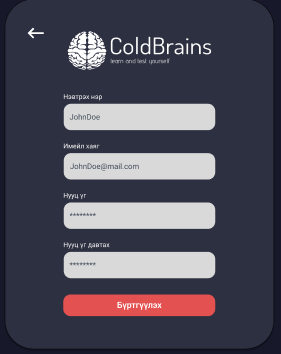
\includegraphics[width=5cm]{img/mockup/register.PNG}
  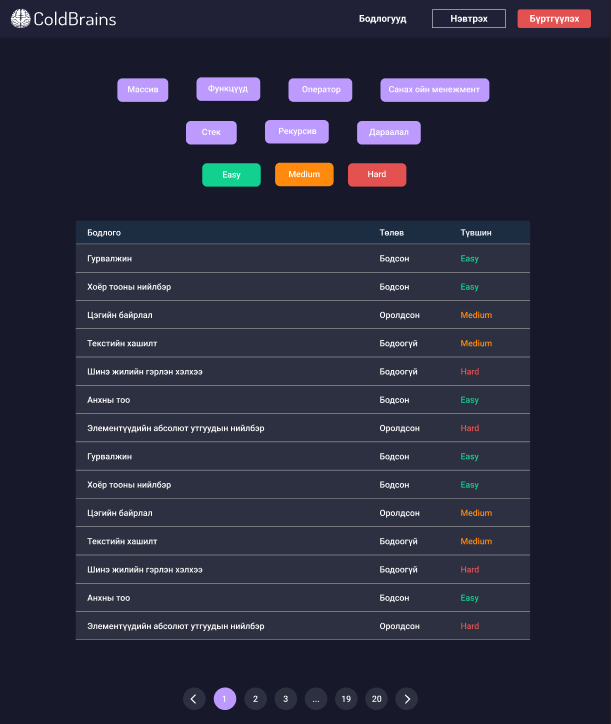
\includegraphics[width=5cm]{img/mockup/problems.PNG}
  \caption{Mockup}
\end{figure}

\clearpage

Wireframe-ийг илүү дэлгэрэнгүй \cite{wireframe}-с харах боломжтой. Нэвтрэх, бүртгүүлэх, бодлогууд, профайл, бодолт, хариунууд, хариу зэрэг интерфейсүүдийг зохиомжилсон.

Өнгөний сонголтуудыг \textbf{Visual Studio Code} код засварлагчийн хамгийн түгээмэл сонголтууд\cite{VSC theme} болон \textbf{Programming Color Palette}-ээс сэдэвлэн оноож өгсөн билээ.

\section{Технологиуд болон шийдлүүд}
\subsection{NEXTjs хувилбар 13}
NEXTjs нь React сангийн фреймворк бөгөөд хамгийн түгээмэл хэрэглэгддэг интерактив фреймворк юм. Хэрэглэгчийн интерфейсийг хэрэгжүүлэхэд хамгийн өргөн сонголтууд болон том экосистем\footnotemark{}тэйгээрээ бусад технологиудаасаа илүү байж чаддаг билээ.\footnotetext{Тухайн технологитой холбоо бүхий мэдээлэл, хэрэглээний бодит жишээ, заах арга зүйн нэгдэл} NEXTjs-ийн тус-ламжтайгаар хэрэглэгчийн интерфейсийг интерактив олон компонентуудад хувааж, хэрэглэг-чийн үйл ажиллагааг хянах боломжтой. 

NEXTjs-ийн хувилбар 13-ыг ашигласнаар дата дамжуулах болон сервер талдаа компонен-туудыг зурах, cache хийх аргачлал зэрэг илүү хөгжүүлэгчид хялбар байх бөгөөд маш олон түгээмэл ашиглагддаг сан, package-ууд нь NEXTjs/React-д зориулан нийтлэгдсэн байдаг.

\subsection{Next.js auth}
Энэхүү сан нь NEXTjs дээр \textbf{session control} хийхэд хамгийн тохиромжтой бөгөөд хэрэглэгчид зориулсан JWT(Json Web Token) токеныг бэлдэж cookie дээр байршуулж, мөн гадны олон түгээмэл системүүдтэй хэрэглэгчийн нээлттэй датаг хуваалцах боломжийг олгодог. Үүний Google, Github зэрэг мэдээллээр хангагчтай харьцах боломж бүхий хэсгийг NEXTjs дээр амархан ашиглах боломжтой. Хэрэглэгчийн нэвтрэх токенг cookie байдлаар хадгалж тухайн токеноос хэрэглэгчийн мэдээллийг decrypt хийж ашиглах боломжоор хангаж өгдөг. 

\subsection{MUI дизайн}
Material UI нь Google-ийн Material дизайныг хэрэгжүүлдэг React компонентуудын сан юм. Интерфейс хэрэгжүүлдэг frontend инженерүүдийн хувьд цагийг хэмнэсэн түгээмэл багаж бөгөөд React-ийн \textbf{Server Side Rendering}-ийг дэмждэг билээ. 

Цаашлаад богино хугацаанд өөрийн өнгөний загварчилгаа(customization) бүхий Responsive интерфейсийг хэрэгжүүлэхэд тусалдаг билээ. Одоогоор React-ийн хамгийн олон хэрэглэгчтэй сан гэж тодорхойлогддог билээ. 

\subsection{Codemirror}
Codemirror гэх энэхүү javascript UI(хэрэглэгчийн интерфейс) бүхий сан нь "Coldbrains"-д гол тоглогчийн үүргийг гүйцэтгэж байгаа бөгөөд энэхүү сангийн тухай дурьдвал
7 хоног бүр 2-3 сая гаруй таталттай байдаг\cite{codemirrorinfo}.   

\begin{figure}[h]
  \centering
  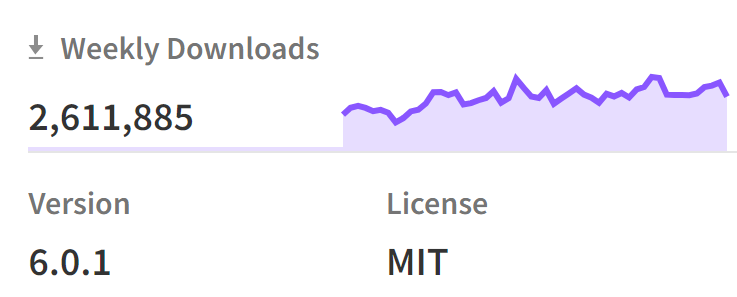
\includegraphics{img/codemirror-npm.PNG}
  \caption{Codemirror сан}
\end{figure}

Цаашлаад Microsoft-ийн Monaco Editor(Visual Studio Code дээр ашиглагддаг), Tern.js зэрэг сангуудын тусламжтайгаар Intellisense бүхий код засварлагчийг бий болгох боломжтой,  өөрөө тухайн код бичигчдээ зориулан extension\footnotemark{} \footnotetext{Боломжит өргөтгөл}-үүдийг бичиж өгөх боломжтой бөгөөд олон төрлийн платформуудыг дэмждэг билээ. 

"Coldbrains" систем дээр энэхүү Codemirror сан нь маш хэрэгтэй хэрэглэгчийн интерфейсийн үүргийг гүйцэтгэж байгаа бөгөөд Codemirror сан дээр бичсэн uiw/react-codemirror сан нь энэхүү хэрэглээг илүү уян хатан болгож, олон хэлний синтакс болон олон өнгөний сонголт зэрэг боломжуудыг бий болгож байгаа. Код засварлагчийн болон хэрэглэгчийн интерфейсийг уян хатан байдлаар хэрэгжүүлэхэд энэхүү \hyperlink{https://uiwjs.github.io/react-codemirror/}{@uiw/codemirror} шийдэл болж байгаа.

\subsection{AWS болон Firebase}
Хэрэглэгчийн кодыг функциональ програмчлалын аргаар зохиомжлогдсон сервер дээр ажиллуулах бөгөөд энэ нь AWS-ийн Lambda буюу stateless байдлаар ажилладаг серверт тохиромжтой. AWS нь тухайн хүсэлтийг хүлээж аван тодорхой холбоо үүсгэх ба handshake хийлгүйгээр REST API-аар Firebase-ийн Firestore NoSQL өгөгдлийн сан руу дата дамжуулах билээ. 

AWS lambda нь хүсэлт ирэх үед хамгийн хурдан хариу өгөхийн тулд Cold start\footnotemark{} \footnotetext{Эхнээс нь бүр мөсөн асаах} хийхээс сэргийлж хамгийн сүүлд ажиллагаатай байсан container-ийг ашигладаг бөгөөд тухайн container-ууд ажиллагаанд ороогүй удсан тохиолдолд нөөцийг хэмнэн өөрийн санах ойг цэвэрлэдэг байна. 

Singapore дээр байрлах серверийг ашигласан болно. Firestore 50000 уншилт/сар, 20000 бичилт/сард үнэгүй ашиглах боломжийг олгодог. AWS lambda нь мөн адил бөгөөд MVP(Minimum viable product)-ийг хэрэгжүүлэхэд эдгээр платформууд нь хамгийн тохиромжтой гэж үзсэн.

\subsection{Хэрэглэгчийн кодыг ажиллуулах}
Хэрэглэгчийн кодыг хэл тус бүр дээр аюулгүй ажиллагаан үүднээс AWS-ийн lambda серверийг ашиглаж байгаа. Эдгээр нь
\begin{enumerate}
  \item Python - python-shell
  \item C/C++ - emscripten
  \item Javascript - javascript virtual machine 2
\end{enumerate}
зэрэг сан болон технологиудыг кодыг ажиллуулахаар ашигласан байгаа билээ. Эдгээр нь customizable буюу оролт/гаралт, ашиглах боломжтой сангууд, ажиллах хугацааны хязгаарлалтуудыг тус тус дэмждэг бөгөөд AWS lambda сервер дээр байршуулснаар тухайн серверийн нөөцийн хуваарилалтыг шийдэж өгч байгаа билээ. 

\subsection{Bcrypt}
bcrypt нь "Blowfish" болон "crypt" гэх 2 үгнээс үүдэлтэй бөгөөд өмнөх UNIX нууц үгийн системийн crypt технологиос үндэслэн бий болсон функц билээ\cite{bcrypt}. Одоогоор нууц үгийг hash хийхэд түгээмэл хэрэглэгдэж буй энэхүү функц нь hash хийхэд ашиглаж буй хугацаагаараа харьцангуй удаан гэдгээрээ ялгардаг бөгөөд аливаа гадны этгээдэд brute-force attack хийхээс сэргийлж байгаа билээ. Энэхүү функц нь одоогийн технологийн чадалд нийцэх бөгөөд супер компьютеруудад болон ирээдүйд гарч ирэх технологийн хөгжлөөс үүдэн аюулгүй байдлыг бүрэн хангаж чадахгүй байх эрсдэлтэй. Bcrypt нь salt буюу нэмэлт encrypt хийх тэмдэгт мөрүүдийг ашигладаг. "Coldbrains" системийн хувьд хэрэглэгчийг бүртгэх болон нэвтэрч ороход энэхүү функцийг ашиглаж байгаа билээ.

\subsection{ExpressJS}
Хүсэлтийг Nodejs орчинд боловсруулахыг дэмждэг энэхүү фреймворк нь экосистем баялаг байдгаараа олон асуудлуудын шийдэл болж өгдөг. Үүн дээр үндэслэн үүссэн NestJS, Sails.js, Restify зэрэг олон технологиуд байдаг бөгөөд "Coldbrains" системд middleware-уудыг нь түлхүү ашигласан билээ. 
\begin{enumerate}
  \item throttling - Хүсэлтийн тоог тодорхой хугацааны завсарт хязгаарлаж өгдөг бөгөөд \textbf{express-rate-limit} санг орж ирж буй хүсэлтүүдийн IPv4 хаягаар танин хязгаарладаг. Ихэвчлэн серверийн ачааллыг бууруулах, нөөцийг хэмнэх, хэрэгцээгүй тооцооллыг багасгах зорилгоор ашиглагддаг. 
  \item route - ExpressJS-ийн хүсэлтүүдийг боловсруулах модиулуудад хуваах боломжтой. Энэ нь программистуудын хувьд илүү цэгцтэй хамтын ажиллагааг дэмжиж өгдөг билээ.
\end{enumerate}

\subsection{Caching}
Уншилт бичилтээр хязгаарлагдах шийдэлд хамгийн хэрэгцээт зүйл нь хэрэглэгчийн статик хэрэгцээт өгөгдлүүдийг \textit{Cache} хийх байдаг. NEXTjs-ийн 13 хувилбар нь javascript хэлний \textbf{fetch} функцийг дахин тодорхойлж, хэрэгцээт датаг өгөгдлийн сангаас биш сервер дээр үүсгэн хадгалах боломжийг олгодог. Эдгээр давуу талуудыг Vercel платформ нь дэмжиж, хэрэглэгчид тодорхой цагийн завсарт ижил өгөгдлийг дамжуулж өгдөг. Ингэснээр тухайн Firebase-ийн шийдлийг илүү үр дүнтэйгээр ашиглах боломжтой бөгөөд хэрэглэгчийнхээ тоог үржүүлэ нэмэгдүүлэх боломжийг олгоно. 

NEXTjs-ийн caching техникийг ашигласнаар "Coldbrains" нь Firebase-ээс өдөртөө зөвхөн ганцхан уншилт хийгээд бодлогуудын мэдээллийг авах боломжтой болох юм. Хэрэглэгч бодолтоо харахын тулд мөн хугацааны интервал буюу 5 минут тутамд шинээр татагдаж cache болж буй өгөгдлөөс харах боломжтой. Ингэснээр 1440 / 5 = 288 уншилт/өдөр хамгийн ихдээ хийх билээ.

\section{Өгөгдлийн сангийн зохиомж}
Өгөгдлийн сан нь NoSQL бөгөөд Firebase-ийн Firestore өгөгдлийн санг ашигласан болно. Тухайн өгөгдлийн сан нь \textbf{collection}, \textbf{document} зэргээр өгөгдлийг загварчилдаг бөгөөд дотроо collection нь олон document-үүдийн цуглуулгыг илэрхийлнэ. Мөн collection нь document-ийг агуулах төдийгүй document нь өөртөө collection харъяалуулах боломжтой бөгөөд түүнийг subcollection гэж нэрлэдэг. 

Firestore-ийн document нь өөрийн дотроо collection-г агуулахгүй хэдий ч тухайн collection-ийн заагч байдлаар оршиж болдог билээ. Document-д заагдсан collection-г \textbf{subcollection} гэж Firebase платформ дээр тодорхойлсон байдаг\cite{datamodeling}.

\clearpage